\documentclass[11pt,a4paper]{article}
\usepackage[utf8]{inputenc}
\usepackage[T1]{fontenc}
\usepackage[brazil]{babel}
\usepackage{lmodern}
\usepackage[margin=2.5cm]{geometry}
\usepackage{amsmath,amssymb}
\usepackage{graphicx}
\usepackage{booktabs}
\usepackage{tabularx}
\usepackage{caption}
\usepackage{float}
\usepackage{setspace}
\usepackage{microtype}
\usepackage{xcolor}
\usepackage[round,authoryear]{natbib}
\usepackage[colorlinks=true,linkcolor=blue!50!black,citecolor=blue!50!black,urlcolor=blue!50!black]{hyperref}
\captionsetup{font=small,labelfont=bf,justification=centering}
\newcommand{\nota}[1]{\par\vspace{2pt}\begin{minipage}{\linewidth}\footnotesize\textit{Nota}: #1\end{minipage}}
\onehalfspacing

\title{\textbf{Mais armas, mais homicídios? A flexibilização do acesso a armas de fogo no Brasil e a violência letal nos municípios e na fronteira da soja (2015--2024)}}
\author{Ricardo Alves dos Santos\thanks{Universidade do Estado de Mato Grosso (UNEMAT), Programa de Pós-Graduação em Propriedade Intelectual e Transferência de Tecnologia para a Inovação (PROFNIT). Autor correspondente. E-mail: \href{mailto:ricardo.alves@unemat.br}{ricardo.alves@unemat.br}.}
\and Cleiton Franco\thanks{Universidade do Estado de Mato Grosso (UNEMAT), Programa de Pós-Graduação em Propriedade Intelectual e Transferência de Tecnologia para a Inovação (PROFNIT), Sinop, MT.}
\and Wylmor Dalfovo\thanks{Universidade do Estado de Mato Grosso (UNEMAT), Programa de Pós-Graduação em Propriedade Intelectual e Transferência de Tecnologia para a Inovação (PROFNIT).}
\and Lindomar Pegorini\thanks{Universidade do Estado de Mato Grosso (UNEMAT), Programa de Pós-Graduação em Propriedade Intelectual e Transferência de Tecnologia para a Inovação (PROFNIT).}}
\date{Novembro de 2026}

\begin{document}
\maketitle
\thispagestyle{empty}

\begin{abstract}
\noindent Entre 2019 e 2022, uma sequência de decretos federais flexibilizou o acesso a armas de fogo no Brasil, e os novos registros de armas por civis chegaram a mais que dobrar. Este artigo estima o efeito dessa expansão sobre os homicídios por arma de fogo, combinando, para os 5.570 municípios brasileiros entre 2015 e 2024, os registros de armas do Sistema Nacional de Armas (SINARM) com os óbitos do Sistema de Informações sobre Mortalidade. A identificação explora a variação municipal na intensidade do choque em desenhos de diferenças em diferenças com tratamento contínuo, adoção escalonada \citep{callaway2021} e controle sintético \citep{arkhangelsky2021}. Cada novo registro por mil habitantes em 2019--2022 eleva a taxa de homicídios por arma de fogo em 0{,}225 por 100 mil habitantes, e os municípios que experimentaram um salto de registros apresentam, em média, 1{,}62 óbitos adicionais por 100 mil. O efeito restringe-se às mortes por arma de fogo, não se observa em homicídios por arma branca e é mais intenso na fronteira da soja, onde atinge 2{,}37 óbitos por 100 mil. Os resultados são sensíveis à escolha do grupo de comparação no estimador de controle sintético, e não há indícios de reversão após a restrição de 2023.

\vspace{0.6em}
\noindent\textbf{Palavras-chave}: armas de fogo; homicídios; diferenças em diferenças; controle sintético; fronteira agrícola; Brasil.

\noindent\textbf{Classificação JEL}: K42; I18; C23; R11; Q15.
\end{abstract}

\newpage
\setcounter{page}{1}

\section{Introdução}

Entre 2019 e 2022, o Brasil atravessou a mais profunda alteração no controle de armas de fogo desde o Estatuto do Desarmamento (Lei nº 10.826/2003). Uma sequência de decretos presidenciais e de portarias do Comando do Exército flexibilizou a comprovação de efetiva necessidade para a posse de armas por civis, elevou os limites de aquisição de armas e munições e estendeu o acesso a calibres restritos aos caçadores, atiradores desportivos e colecionadores (CACs). O número de certificados de registro de CACs ativos passou de 117.467 em 2018 para 783.385 em 2022 \citep{fbsp2023}, e os novos registros de armas de fogo por civis no SINARM passaram de cerca de 75 mil por ano em 2018--2019 para 165 mil em 2021. A partir de 2023, os Decretos nº 11.366 e nº 11.615 reverteram parte dessas medidas.

O efeito de uma expansão dessa magnitude sobre a violência letal é teoricamente ambíguo. No modelo de escolha racional de \citet{becker1968}, a maior probabilidade de a vítima estar armada eleva o custo esperado do crime e pode ter efeito dissuasório. Ao mesmo tempo, um estoque maior de armas em circulação torna mais letais os conflitos interpessoais e facilita o desvio de armas para o mercado ilegal. A evidência internacional tende a favorecer o segundo canal \citep{duggan2001,cook2006}, e a experiência brasileira com o Estatuto do Desarmamento aponta na mesma direção \citep{souza2007,cerqueira2012}. Para o ciclo recente de flexibilização, contudo, as evidências disponíveis são agregadas por região ou estado \citep{baculi2021,wakim2025} e não exploram a variação entre municípios na intensidade com que o choque regulatório se materializou.

Este artigo estima o efeito da expansão dos registros de armas sobre os homicídios por arma de fogo em todos os 5.570 municípios brasileiros entre 2015 e 2024. A medida de exposição é construída a partir dos microdados abertos do SINARM, que registram cada arma por município, mês e categoria do proprietário, e os resultados vêm do Sistema de Informações sobre Mortalidade (SIM). A estratégia empírica combina diferenças em diferenças com tratamento contínuo, o estimador de \citet{callaway2021} para adoção escalonada e o \textit{synthetic difference-in-differences} (SDID) de \citet{arkhangelsky2021}. Uma tripla diferença que compara homicídios por arma de fogo e por arma branca no mesmo município e ano isola o canal da disponibilidade de armas. O trabalho examina ainda a fronteira da soja, onde a expansão recente da área plantada se combina com o desmatamento e com uma demanda elevada por autodefesa armada, motivado pela evidência de que a expansão da soja elevou os homicídios no país \citep{moreno2024}.

Os resultados indicam que a flexibilização elevou os homicídios por arma de fogo. Na especificação principal, cada novo registro por mil habitantes eleva a taxa em 0{,}225 óbitos por 100 mil habitantes ao ano (erro-padrão de 0{,}092), o que equivale a 0{,}92 óbitos por 100 mil entre o primeiro e o terceiro quartil de exposição. O estimador de \citet{callaway2021} produz um efeito médio de 1{,}62 óbitos por 100 mil nos municípios que experimentaram um salto de registros. O efeito é específico às mortes por arma de fogo e é maior na fronteira da soja (2{,}37 por 100 mil). Os coeficientes pré-tratamento do \textit{event study} convencional não são nulos em conjunto, e o SDID é sensível à definição do grupo de comparação; esses limites são discutidos em detalhe.

O artigo contribui para a literatura de três maneiras. Primeiro, fornece a primeira estimativa causal, em nível municipal, dos efeitos da flexibilização de 2019--2022. Segundo, constrói um painel reprodutível que integra quatro bases públicas (SINARM, SIM, IBGE e MapBiomas). Terceiro, aplica o SDID à avaliação de políticas de armas, como recomendado por \citet{benmichael2024}, e documenta a heterogeneidade territorial do efeito associada à expansão da soja. A Seção~\ref{sec:contexto} descreve a intervenção; a Seção~\ref{sec:dados} apresenta os dados; a Seção~\ref{sec:estrategia} discute a estratégia empírica; as Seções~\ref{sec:resultados} a \ref{sec:soja} apresentam os resultados; a Seção~\ref{sec:conclusao} conclui.

\section{Contexto institucional}\label{sec:contexto}

O Estatuto do Desarmamento condicionou a posse de armas por civis à comprovação de efetiva necessidade, avaliada pela Polícia Federal. O Decreto nº 9.685, de janeiro de 2019, passou a presumir essa necessidade para residentes em áreas rurais e em estados com mais de 10 homicídios por 100 mil habitantes, critério atendido, na prática, por todas as unidades da federação. Os Decretos nº 9.785, nº 9.845 e nº 9.846, de 2019, ampliaram os limites de aquisição de munições e o rol de armas permitidas, e os Decretos nº 10.627 a nº 10.630, de 2021, elevaram o número de armas por proprietário. O Decreto nº 11.366, de janeiro de 2023, e o Decreto nº 11.615, de julho de 2023, reverteram parte dessas medidas.

A Figura~\ref{fig:mensal} mostra a resposta mensal dos registros. Até 2019, os novos registros de armas por civis oscilavam entre 4 e 8 mil por mês. A aceleração ganhou força a partir de meados de 2020, atingiu o pico em 2021, com até 16 mil registros mensais, e desapareceu a partir do fim de 2022, quando os registros se estabilizaram em torno de 2 mil por mês. A defasagem entre os decretos de 2019 e a aceleração de 2020 indica que o choque se materializou gradualmente e com intensidade distinta entre municípios, o que motiva a medida de exposição acumulada entre 2019 e 2022 e a definição de coortes pelo primeiro salto de registros de cada município.

\begin{figure}[H]
\centering
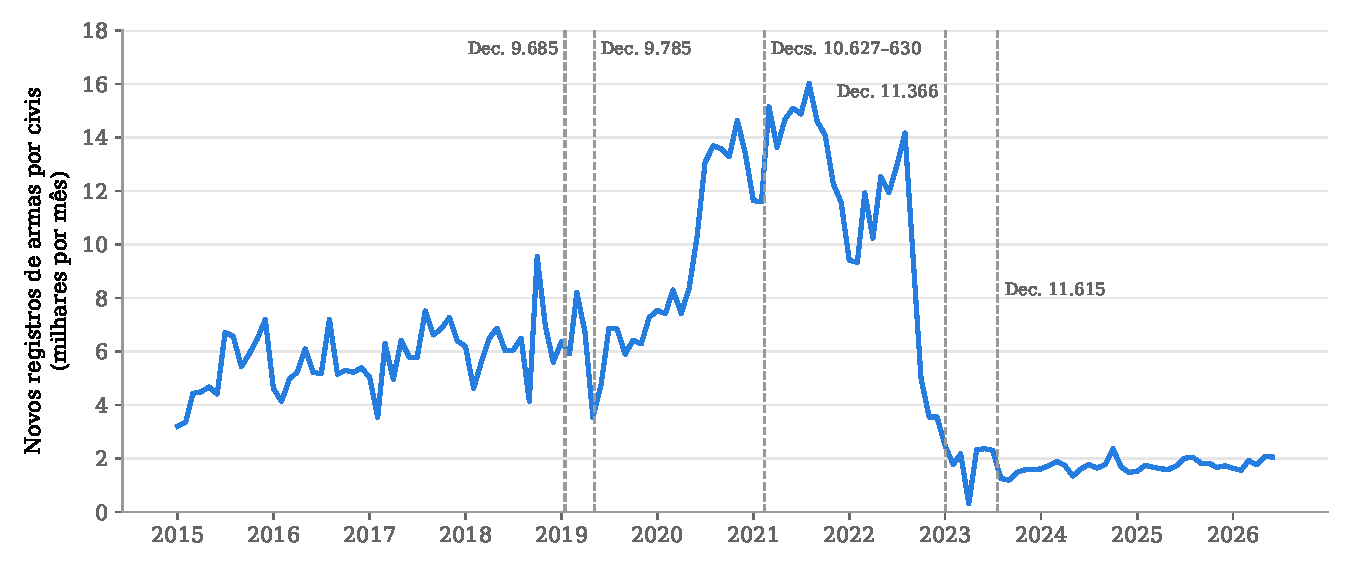
\includegraphics[width=\linewidth]{figs/registros_mensais_pt.pdf}
\caption{Novos registros mensais de armas de fogo por civis no Brasil e marcos regulatórios}\label{fig:mensal}
\nota{Soma nacional dos registros da categoria ``Cidadão'' no SINARM por mês de emissão, de janeiro de 2015 a junho de 2026. Fonte: elaboração própria a partir do SINARM/Polícia Federal.}
\end{figure}

\section{Dados}\label{sec:dados}

O painel cobre os 5.570 municípios brasileiros entre 2015 e 2024, com 55.700 observações e quatro anos anteriores à intervenção. A exposição ao tratamento vem dos dados abertos do SINARM, mantidos pela Polícia Federal, que registram cada arma de fogo por ano e mês de emissão, município e categoria do proprietário. Utilizam-se os registros da categoria ``Cidadão'', que correspondem às armas de posse de civis e são o objeto direto dos decretos de 2019. Os registros de CACs, mantidos pelo Exército no Sistema de Gerenciamento Militar de Armas (SIGMA), não são divulgados por município. Os dados provêm da Polícia Federal \citep{sinarm}, do Ministério da Saúde \citep{sim}, do IBGE \citep{ibge} e do Projeto MapBiomas \citep{mapbiomas}. Dos 979.601 registros emitidos entre 2015 e 2025, 99,99\% foram associados a um código municipal do IBGE. A soma dos novos registros entre 2018 e 2022 por unidade da federação tem correlação de 0,89 com o aumento do estoque de registros ativos publicado pelo \citet{fbsp2023}.

A intensidade do tratamento é definida como
\begin{equation}
\Delta REG_i = \frac{\text{novos registros por civis em 2019--2022}_i}{\text{população em 2018}_i}\times 1.000.
\end{equation}
Os óbitos provêm dos microdados do SIM, agregados por município de residência: homicídios por arma de fogo (CID-10 X93--X95), por arma branca (X99) e por outros meios (X85--X92, X96--X98, Y00--Y09), além de óbitos em acidentes de transporte terrestre (V01--V89) e por COVID-19 (B34.2). As taxas são expressas por 100 mil habitantes, com população das estimativas do IBGE e do Censo de 2022. Os controles incluem o logaritmo do valor adicionado bruto da agropecuária per capita, deflacionado pelo IPCA, o logaritmo da densidade demográfica e a mortalidade por COVID-19. A fronteira agrícola ativa reúne os municípios cujo desmatamento entre 2015 e 2018, em proporção da área municipal, supera a mediana nacional, segundo a Coleção 11 do MapBiomas.

A Tabela~\ref{tab:desc} apresenta as estatísticas descritivas. A fronteira agrícola absorveu o choque com mais intensidade (Figura~\ref{fig:grupos}), mas os homicídios por arma de fogo caíram em ambos os grupos após 2018, acompanhando a tendência nacional. A pergunta empírica é, portanto, se essa queda foi menor onde mais armas entraram em circulação. A Figura~\ref{fig:quartis} sugere que sim: até 2018 os municípios do quartil superior de expansão dos registros tinham taxas próximas às do quartil inferior; entre 2019 e 2023, passaram a apresentar taxas mais altas, diferença que praticamente desaparece em 2024.

\begin{table}[H]
\centering\footnotesize\setlength{\tabcolsep}{4pt}
\caption{Estatísticas descritivas por grupo territorial e período}\label{tab:desc}
\begin{tabular}{lcccc}
\toprule
 & \multicolumn{2}{c}{Consolidados} & \multicolumn{2}{c}{Fronteira agrícola} \\
\cmidrule(lr){2-3}\cmidrule(lr){4-5}
 & 2015--18 & 2019--24 & 2015--18 & 2019--24 \\
\midrule
Intensidade $\Delta REG_i$ (registros por mil hab.) & 3{,}87 (5{,}36) & 3{,}87 (5{,}36) & 3{,}84 (5{,}38) & 3{,}84 (5{,}37) \\
Novos registros por mil hab. por ano & 0{,}60 (1{,}08) & 0{,}70 (1{,}34) & 0{,}44 (0{,}96) & 0{,}70 (1{,}36) \\
Homicídios por arma de fogo (por 100 mil) & 11{,}37 (18{,}10) & 9{,}89 (16{,}57) & 16{,}20 (20{,}22) & 14{,}54 (18{,}53) \\
Homicídios por arma branca (por 100 mil) & 4{,}35 (8{,}24) & 3{,}74 (7{,}70) & 5{,}07 (8{,}51) & 4{,}55 (8{,}24) \\
Óbitos no trânsito (por 100 mil) & 23{,}32 (22{,}79) & 23{,}08 (22{,}91) & 24{,}11 (21{,}47) & 23{,}68 (21{,}65) \\
Homicídios por arma de fogo, taxa agregada & 18{,}42 & 12{,}44 & 24{,}29 & 17{,}93 \\
Municípios & 2.785 & 2.785 & 2.785 & 2.785 \\
\bottomrule
\end{tabular}
\nota{Médias simples entre municípios, com desvios-padrão entre parênteses; a penúltima linha apresenta a taxa agregada do grupo (óbitos totais sobre população total). Fronteira agrícola: desmatamento entre 2015 e 2018 acima da mediana nacional. Fontes: SINARM/PF, SIM/DATASUS, IBGE e MapBiomas.}
\end{table}

\begin{figure}[H]
\centering
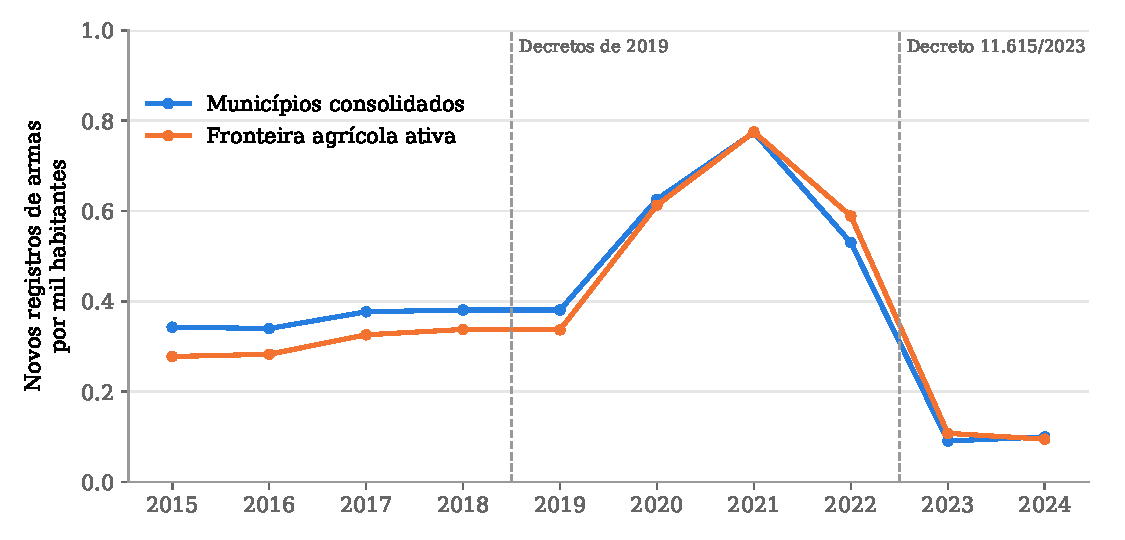
\includegraphics[width=0.78\linewidth]{figs/registros_grupos_pt.pdf}
\caption{Novos registros de armas por civis por mil habitantes, por grupo territorial}\label{fig:grupos}
\nota{Taxas agregadas por grupo. Fontes: SINARM/PF e IBGE.}
\end{figure}

\begin{figure}[H]
\centering
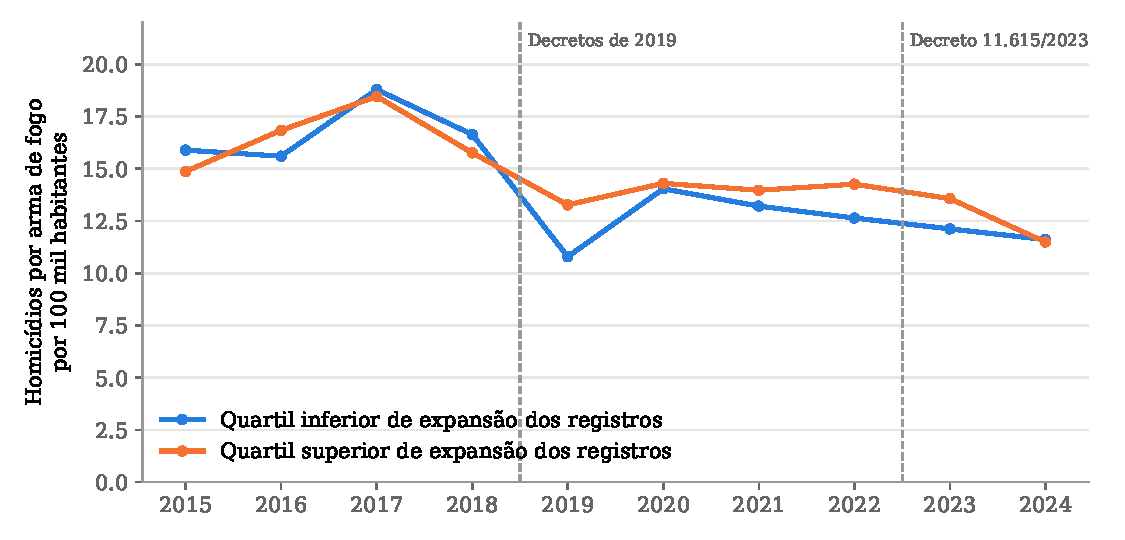
\includegraphics[width=0.78\linewidth]{figs/homicidios_quartis_pt.pdf}
\caption{Homicídios por arma de fogo por quartil de expansão dos registros}\label{fig:quartis}
\nota{Taxas agregadas dos municípios do primeiro e do quarto quartil de $\Delta REG_i$. Fontes: SIM/DATASUS, SINARM/PF e IBGE.}
\end{figure}

\section{Estratégia empírica}\label{sec:estrategia}

Como os decretos alcançaram todo o território nacional ao mesmo tempo, a identificação explora a variação entre municípios na intensidade com que o choque se materializou. A especificação principal é
\begin{equation}\label{eq:twfe}
Y_{it} = \alpha_i + \lambda_t + \beta\,(\Delta REG_i \times Pos_t) + X_{it}'\gamma + \varepsilon_{it},
\end{equation}
em que $Y_{it}$ é a taxa de homicídios por arma de fogo do município $i$ no ano $t$, $\alpha_i$ e $\lambda_t$ são efeitos fixos de município e de ano, $Pos_t$ indica os anos a partir de 2019 e $X_{it}$ reúne os controles. O parâmetro $\beta$ mede o efeito de um novo registro por mil habitantes sobre a taxa de homicídios por arma de fogo. As regressões são ponderadas pela população, e os erros-padrão são agrupados por município. Estima-se também um modelo de Poisson com efeitos fixos para as contagens de óbitos, com o logaritmo da população como \textit{offset}, e versões que incluem as interações $\Delta REG_i \times Pos_t \times Fronteira_i$ e $\Delta REG_i \times Pos2023_t$.

A hipótese de identificação é a de que, na ausência dos decretos, municípios com expansão alta e baixa de registros teriam seguido trajetórias paralelas de homicídios por arma de fogo. Para avaliá-la, estima-se o \textit{event study}
\begin{equation}
Y_{it} = \alpha_i + \lambda_t + \sum_{t\neq 2018}\delta_t\,(\Delta REG_i\times \mathbf{1}[\text{ano}=t]) + X_{it}'\gamma + \varepsilon_{it}.
\end{equation}
Como o momento em que cada município absorveu o choque variou e o estimador de efeitos fixos bidirecionais pode ser viesado sob efeitos heterogêneos \citep{goodmanbacon2021,dechaisemartin2020,sun2021}, utiliza-se também o estimador de \citet{callaway2021}. As coortes são definidas pelo primeiro ano entre 2019 e 2021 em que a taxa anual de registros do município atingiu ao menos o dobro de sua média de 2015--2018, o que gera 1.006 municípios na coorte de 2019, 1.355 na de 2020 e 878 na de 2021, com 2.331 municípios nunca tratados.

Duas estratégias adicionais enfrentam as principais ameaças à identificação. A tripla diferença
\begin{equation}
Y_{imt} = \alpha_{im} + \lambda_{mt} + \theta_{it} + \beta_{DDD}\,(\Delta REG_i\times AF_m\times Pos_t) + \varepsilon_{imt},
\end{equation}
em que $m$ indexa o meio empregado no homicídio, compara homicídios por arma de fogo e por arma branca no mesmo município e ano e absorve, por meio de $\theta_{it}$, qualquer choque local que afete a violência em geral. O SDID de \citet{arkhangelsky2021} reconstrói a trajetória pré-tratamento dos municípios tratados com pesos de unidades e de tempo e exige tratamento binário com adoção em bloco. Os grupos são definidos de três formas: quartil superior contra quartil inferior de $\Delta REG_i$, coorte de 2019 contra municípios nunca tratados e fronteira da soja contra produtores consolidados. Os erros-padrão do SDID são obtidos por \textit{bootstrap} de municípios com 200 replicações.

\section{Resultados}\label{sec:resultados}

A Tabela~\ref{tab:main} apresenta os resultados principais. Na coluna (2), que inclui os controles, $\hat\beta = 0{,}225$, com erro-padrão de 0{,}092 (p = 0{,}014). Passar do primeiro para o terceiro quartil de exposição (de 0{,}67 para 4{,}75 registros por mil habitantes) eleva a taxa de homicídios por arma de fogo em 0{,}92 óbitos por 100 mil, o equivalente a 5{,}3\% da taxa média ponderada de 17{,}24. O modelo de Poisson indica aumento de 1{,}44\% nos homicídios por arma de fogo para cada registro adicional por mil habitantes. A interação com a fronteira agrícola é pequena e não significativa ($-$0{,}096; p = 0{,}470), e o termo associado a 2023 não indica reversão até 2024 (0{,}073; p = 0{,}142). Um desenho alternativo, que trata a fronteira agrícola como grupo tratado, confirma que ela recebeu mais armas (0{,}155 registros adicionais por mil habitantes por ano), mas não detecta diferença nos homicídios ($-$0{,}62; p = 0{,}543), pois a classificação binária agrega municípios com exposições muito distintas.

\begin{table}[H]
\centering\footnotesize\setlength{\tabcolsep}{4pt}
\caption{Efeito da expansão dos registros de armas sobre os homicídios por arma de fogo}\label{tab:main}
\begin{tabular}{lcccccc}
\toprule
 & (1) & (2) & (3) & (4) & (5) & (6) \\
 & TWFE & TWFE & Fronteira & Reversão & Poisson & C\&S \\
\midrule
$\Delta REG_i \times Pos_t$ & 0{,}158$^{*}$ & 0{,}225$^{**}$ & 0{,}279$^{**}$ & 0{,}202$^{**}$ & 0{,}014$^{***}$ & 1{,}62$^{***}$ \\
 & (0{,}092) & (0{,}092) & (0{,}126) & (0{,}088) & (0{,}005) & (0{,}59) \\
$\Delta REG_i \times Pos_t \times Fronteira_i$ &  &  & $-$0{,}096 &  &  &  \\
 &  &  & (0{,}133) &  &  &  \\
$\Delta REG_i \times Pos2023_t$ &  &  &  & 0{,}073 &  &  \\
 &  &  &  & (0{,}050) &  &  \\
\midrule
Controles & Não & Sim & Sim & Sim & Sim & Não \\
EF de município e ano & Sim & Sim & Sim & Sim & Sim & -- \\
Ponderação & Pop. & Pop. & Pop. & Pop. & Offset & Pop. \\
Observações & 55.700 & 55.700 & 55.700 & 55.700 & 50.840 & 55.700 \\
\bottomrule
\end{tabular}
\nota{Variável dependente: homicídios por arma de fogo por 100 mil habitantes; na coluna (5), contagem de óbitos com \textit{offset} igual ao logaritmo da população, e o coeficiente é uma semielasticidade. $\Delta REG_i$ é medido em novos registros por mil habitantes. A coluna (6) apresenta o ATT agregado do estimador de \citet{callaway2021}, com os municípios ainda não tratados como grupo de comparação. Erros-padrão agrupados por município entre parênteses. $^{*}$ p$<$0,10; $^{**}$ p$<$0,05; $^{***}$ p$<$0,01.}
\end{table}

O estimador de \citet{callaway2021} (coluna 6) indica que os municípios que experimentaram um salto de registros apresentam, em média, 1{,}62 homicídios por arma de fogo adicionais por 100 mil habitantes (erro-padrão de 0{,}59; intervalo de 95\% entre 0{,}46 e 2{,}77). O resultado é praticamente idêntico quando o grupo de comparação são os municípios nunca tratados (1{,}68; erro-padrão de 0{,}61).

A Tabela~\ref{tab:es} e as Figuras~\ref{fig:es} e \ref{fig:cs} apresentam a dinâmica do efeito. No \textit{event study} com efeitos fixos bidirecionais, os coeficientes pós-2019 são positivos e significativos em todos os anos e atingem o maior valor em 2022--2023, período de maior estoque acumulado. Os coeficientes de 2015 a 2017 também são positivos, e o teste conjunto rejeita a hipótese de que sejam nulos (F = 2{,}82; p = 0{,}038), o que reflete em parte a queda particularmente acentuada dos homicídios em 2018 nos municípios de maior exposição. No estimador de \citet{callaway2021}, que compara cada coorte com seus próprios anos anteriores ao salto, os coeficientes de $k=-4$ a $k=-1$ não são estatisticamente diferentes de zero, e os efeitos posteriores ao salto são positivos e crescentes.

\begin{table}[H]
\centering\footnotesize\setlength{\tabcolsep}{4pt}
\caption{Estimativas dinâmicas (ano de referência: 2018)}\label{tab:es}
\begin{tabular}{llccccc}
\toprule
 & & \multicolumn{2}{c}{Homicídios por arma de fogo} & \multicolumn{2}{c}{Placebo: trânsito} & C\&S \\
\cmidrule(lr){3-4}\cmidrule(lr){5-6}
Ano & Período & $\hat\delta_t$ & EP & $\hat\delta_t$ & EP & ATT($k$) \\
\midrule
2015 & $k=-4$ & 0{,}164 & (0{,}100) & $-$0{,}068 & (0{,}075) & 0{,}84 (0{,}53) \\
2016 & $k=-3$ & 0{,}229$^{**}$ & (0{,}091) & $-$0{,}034 & (0{,}068) & $-$0{,}41 (0{,}48) \\
2017 & $k=-2$ & 0{,}097 & (0{,}068) & 0{,}105 & (0{,}064) & $-$0{,}43 (0{,}51) \\
2018 (ref.) & $k=-1$ & 0 & -- & 0 & -- & 1{,}00 (0{,}65) \\
2019 & $k=+0$ & 0{,}376$^{***}$ & (0{,}118) & $-$0{,}027 & (0{,}078) & 0{,}90 (0{,}38) \\
2020 & $k=+1$ & 0{,}243$^{**}$ & (0{,}097) & $-$0{,}019 & (0{,}070) & 1{,}52 (0{,}58) \\
2021 & $k=+2$ & 0{,}255$^{**}$ & (0{,}114) & 0{,}142$^{**}$ & (0{,}070) & 1{,}76 (0{,}66) \\
2022 & $k=+3$ & 0{,}421$^{***}$ & (0{,}115) & 0{,}164$^{***}$ & (0{,}059) & 1{,}65 (0{,}72) \\
2023 & $k=+4$ & 0{,}431$^{***}$ & (0{,}119) & 0{,}172$^{***}$ & (0{,}056) & 1{,}65 (0{,}87) \\
2024 & $k=+5$ & 0{,}366$^{***}$ & (0{,}127) & 0{,}140$^{**}$ & (0{,}066) & 3{,}69 (1{,}55) \\
\midrule
Teste conjunto pré (2015--17) &  & F = 2{,}82 & p = 0{,}038 & F = 2{,}81 & p = 0{,}038 &  \\
\bottomrule
\end{tabular}
\nota{\textit{Event study} com efeitos fixos de município e de ano, controles e ponderação pela população; erros-padrão agrupados por município. A última coluna apresenta o ATT do estimador de \citet{callaway2021} por tempo relativo $k$ ao primeiro salto de registros, alinhado à linha com o mesmo $k$, com erro-padrão entre parênteses. $^{*}$ p$<$0,10; $^{**}$ p$<$0,05; $^{***}$ p$<$0,01.}
\end{table}

\begin{figure}[H]
\centering
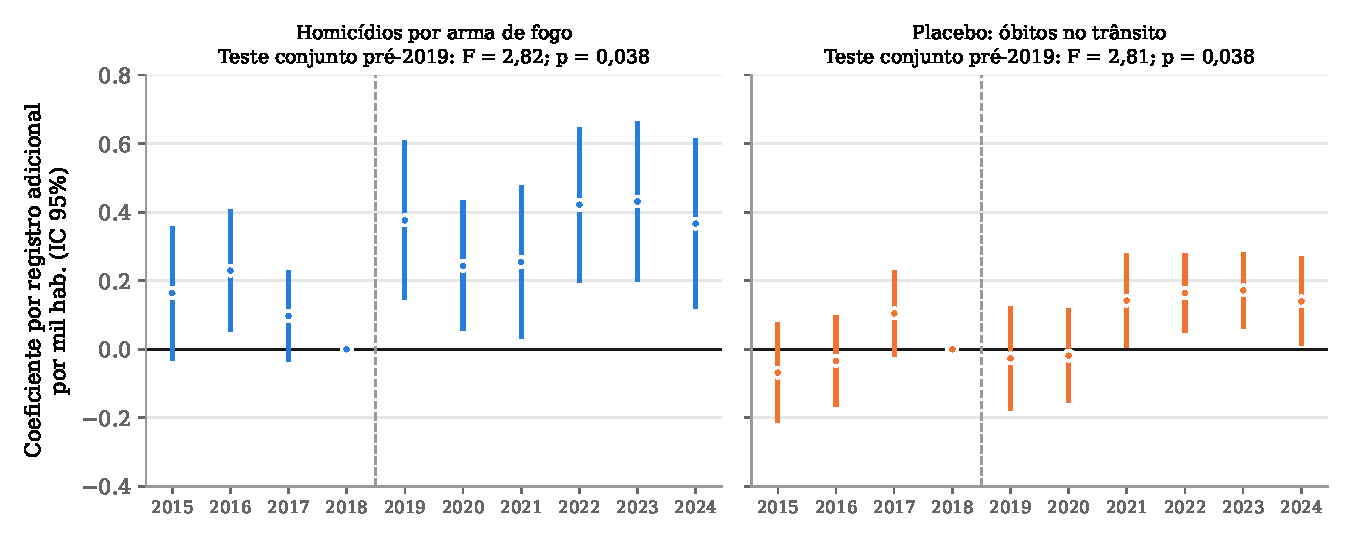
\includegraphics[width=0.95\linewidth]{figs/event_study_pt.pdf}
\caption{\textit{Event study}: coeficientes dinâmicos e intervalos de confiança de 95\%}\label{fig:es}
\nota{Coeficientes por registro adicional por mil habitantes; erros-padrão agrupados por município.}
\end{figure}

\begin{figure}[H]
\centering
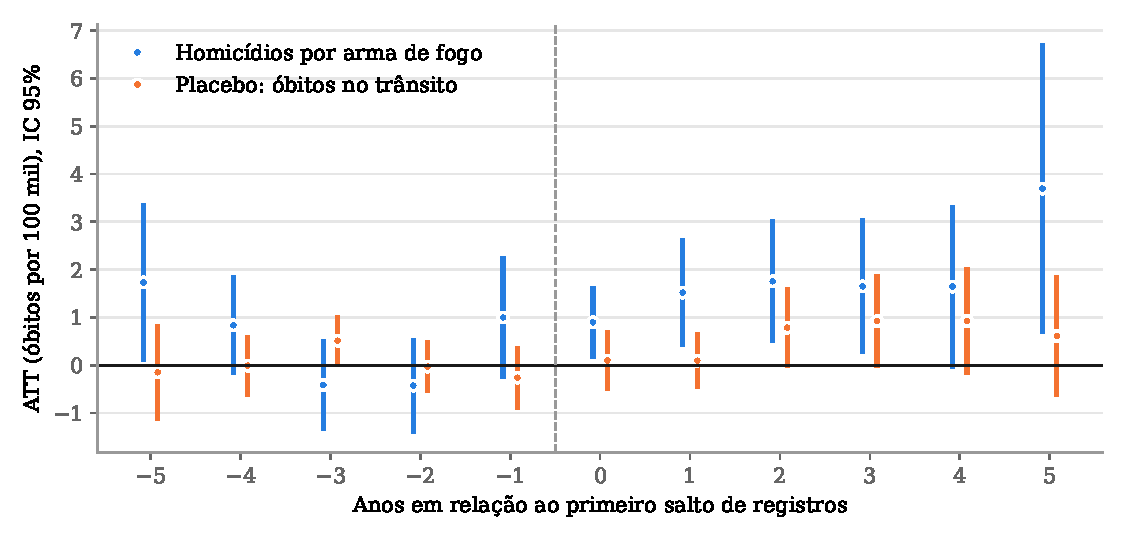
\includegraphics[width=0.75\linewidth]{figs/callaway_santanna_pt.pdf}
\caption{Callaway e Sant'Anna: efeito por tempo relativo ao primeiro salto de registros}\label{fig:cs}
\nota{Grupo de comparação formado pelos municípios ainda não tratados; ponderação pela população; intervalos de confiança de 95\%.}
\end{figure}

\section{Robustez}\label{sec:robustez}

A Tabela~\ref{tab:rob} reúne os testes de robustez. O coeficiente da tripla diferença é positivo e significativo (0{,}190; p = 0{,}032), e os homicídios por arma branca não respondem à expansão dos registros ($-$0{,}013; p = 0{,}413). O aumento da letalidade é, portanto, específico ao meio arma de fogo, o que é coerente com o canal de disponibilidade e afasta explicações baseadas em tendências gerais da violência local. O tratamento binário, definido pelo quartil superior de exposição, produz um efeito de 3{,}88 óbitos por 100 mil. Os controles mais exigentes, que incluem tendências específicas por nível de registros pré-2019 ou efeitos fixos de UF por ano, elevam o coeficiente para cerca de 0{,}54, o que indica que o resultado não decorre de diferenças regionais de tendência. O efeito também se mantém em municípios com 20 mil habitantes ou mais e em cada um dos grupos territoriais.

Dois resultados recomendam cautela. O placebo de resultado com óbitos no trânsito é positivo e significativo no modelo de efeitos fixos (0{,}091; p = 0{,}005), com efeito concentrado em 2021--2024, o que sugere a presença de algum choque concomitante, como o crescimento econômico e do tráfego em municípios do agronegócio que também registraram mais armas. No estimador de \citet{callaway2021}, esse placebo não é significativo (0{,}55; erro-padrão de 0{,}31). O placebo temporal de 2017 é negativo e marginalmente significativo ($-$0{,}154; p = 0{,}071), o que reflete a mesma queda dos homicídios em 2018 observada no \textit{event study}. Por fim, na amostra de 50 municípios, o efeito não é detectável ($-$0{,}024; p = 0{,}915), o que ilustra a importância de utilizar o universo de municípios para estimar efeitos dessa magnitude.

\begin{table}[H]
\centering\small
\caption{Testes de robustez}\label{tab:rob}
\begin{tabular}{lcccc}
\toprule
Especificação & Coeficiente & EP & p-valor & N \\
\midrule
Tripla diferença: arma de fogo vs. arma branca & 0{,}190$^{**}$ & (0{,}088) & 0{,}032 & 111.400 \\
Placebo de resultado: óbitos no trânsito & 0{,}091$^{***}$ & (0{,}032) & 0{,}005 & 55.700 \\
Placebo temporal: choque fictício em 2017 & $-$0{,}154$^{*}$ & (0{,}085) & 0{,}071 & 22.280 \\
Tratamento binário: quartil superior & 3{,}875$^{***}$ & (0{,}806) & $<$0{,}001 & 55.700 \\
Homicídios por arma branca & $-$0{,}013 & (0{,}015) & 0{,}413 & 55.700 \\
Homicídios por outros meios & 0{,}042$^{***}$ & (0{,}011) & $<$0{,}001 & 55.700 \\
Tendências por linha de base de registros & 0{,}536$^{***}$ & (0{,}135) & $<$0{,}001 & 55.700 \\
EF de UF $\times$ ano & 0{,}545$^{***}$ & (0{,}095) & $<$0{,}001 & 55.690 \\
Intensidade em excesso sobre 2015--18 & 0{,}520$^{***}$ & (0{,}134) & $<$0{,}001 & 55.700 \\
Sem ponderação & 0{,}093$^{***}$ & (0{,}024) & $<$0{,}001 & 55.700 \\
Municípios com 20 mil hab. ou mais & 0{,}241$^{***}$ & (0{,}082) & 0{,}003 & 16.520 \\
Subamostra: fronteira agrícola & 0{,}261$^{*}$ & (0{,}144) & 0{,}070 & 27.850 \\
Subamostra: consolidados & 0{,}209$^{*}$ & (0{,}122) & 0{,}087 & 27.850 \\
Amostra de 50 municípios & $-$0{,}024 & (0{,}221) & 0{,}915 & 500 \\
\bottomrule
\end{tabular}
\nota{Todas as regressões incluem efeitos fixos de unidade e de tempo; na tripla diferença, município por meio, ano por meio e município por ano. Salvo indicação, controles e ponderação pela população como na coluna (2) da Tabela~\ref{tab:main}. Erros-padrão agrupados por município. $^{*}$ p$<$0,10; $^{**}$ p$<$0,05; $^{***}$ p$<$0,01.}
\end{table}

A Tabela~\ref{tab:sdid} e a Figura~\ref{fig:sdid} apresentam o SDID. Na comparação entre a coorte de 2019 e os municípios nunca tratados com 20 mil habitantes ou mais, o efeito é de 3{,}32 óbitos por 100 mil (erro-padrão de 0{,}76), com ajuste pré-tratamento quase perfeito. Na comparação entre o quartil superior e o quartil inferior de exposição, porém, o SDID é nulo ($-$0{,}16; erro-padrão de 0{,}89) e torna-se negativo quando os municípios tratados são ponderados pela população ($-$2{,}32; erro-padrão de 0{,}73). Os municípios do quartil inferior concentram-se no Nordeste, cuja dinâmica de homicídios difere da observada no Sul e no Centro-Oeste, onde se concentram os municípios do quartil superior, e quatro anos pré-tratamento oferecem pouca informação para que os pesos sintéticos equilibrem regiões tão distintas. Os placebos com homicídios por arma branca e óbitos no trânsito são nulos. O SDID confirma o efeito quando a comparação é feita entre grupos semelhantes, mas não na comparação entre os extremos da distribuição de exposição, o que recomenda cautela na interpretação da magnitude.

\begin{table}[H]
\centering\footnotesize\setlength{\tabcolsep}{4pt}
\caption{\textit{Synthetic difference-in-differences}}\label{tab:sdid}
\begin{tabular}{lccccccc}
\toprule
Tratados vs. controles & SDID & EP & DiD & EP & SC & EP & N (T/C) \\
\midrule
Q4 vs. Q1, todos & 0{,}03 & (0{,}42) & 0{,}04 & (0{,}42) & $-$0{,}97 & (1{,}84) & 1393/1393 \\
Q4 vs. Q1, tratados pond. pela pop. & $-$2{,}32$^{***}$ & (0{,}73) & $-$2{,}39$^{***}$ & (0{,}77) & $-$1{,}08 & (0{,}84) & 1393/1393 \\
Q4 vs. Q1, $\geq$ 20 mil hab. & $-$0{,}16 & (0{,}89) & $-$0{,}32 & (0{,}93) & $-$1{,}03 & (0{,}90) & 280/465 \\
Q4 vs. Q1, $\geq$ 20 mil, pond. & $-$1{,}77$^{*}$ & (1{,}01) & $-$2{,}09$^{*}$ & (1{,}10) & $-$1{,}38 & (1{,}00) & 280/465 \\
Coorte 2019 vs. nunca tratados & 0{,}27 & (0{,}46) & 0{,}26 & (0{,}45) & $-$0{,}01 & (1{,}14) & 1006/2331 \\
Coorte 2019 vs. nunca, $\geq$ 20 mil & 3{,}32$^{***}$ & (0{,}76) & 3{,}42$^{***}$ & (0{,}75) & 4{,}11$^{***}$ & (0{,}75) & 389/651 \\
\midrule
Placebo arma branca ($\geq$ 20 mil) & $-$0{,}13 & (0{,}25) & $-$0{,}19 & (0{,}26) & 0{,}37 & (0{,}30) & 280/465 \\
Placebo trânsito ($\geq$ 20 mil) & $-$0{,}23 & (0{,}50) & $-$0{,}13 & (0{,}51) & 0{,}80 & (1{,}27) & 280/465 \\
\bottomrule
\end{tabular}
\nota{Variável dependente: homicídios por arma de fogo por 100 mil habitantes. SDID conforme \citet{arkhangelsky2021}, com pesos de unidades e de tempo estimados em 2015--2018 e tratamento a partir de 2019. DiD utiliza pesos uniformes, e SC corresponde ao controle sintético sem pesos de tempo. Erros-padrão por \textit{bootstrap} de municípios (200 replicações). Q4 e Q1 denotam os quartis superior e inferior de $\Delta REG_i$. $^{*}$ p$<$0,10; $^{**}$ p$<$0,05; $^{***}$ p$<$0,01.}
\end{table}

\begin{figure}[H]
\centering
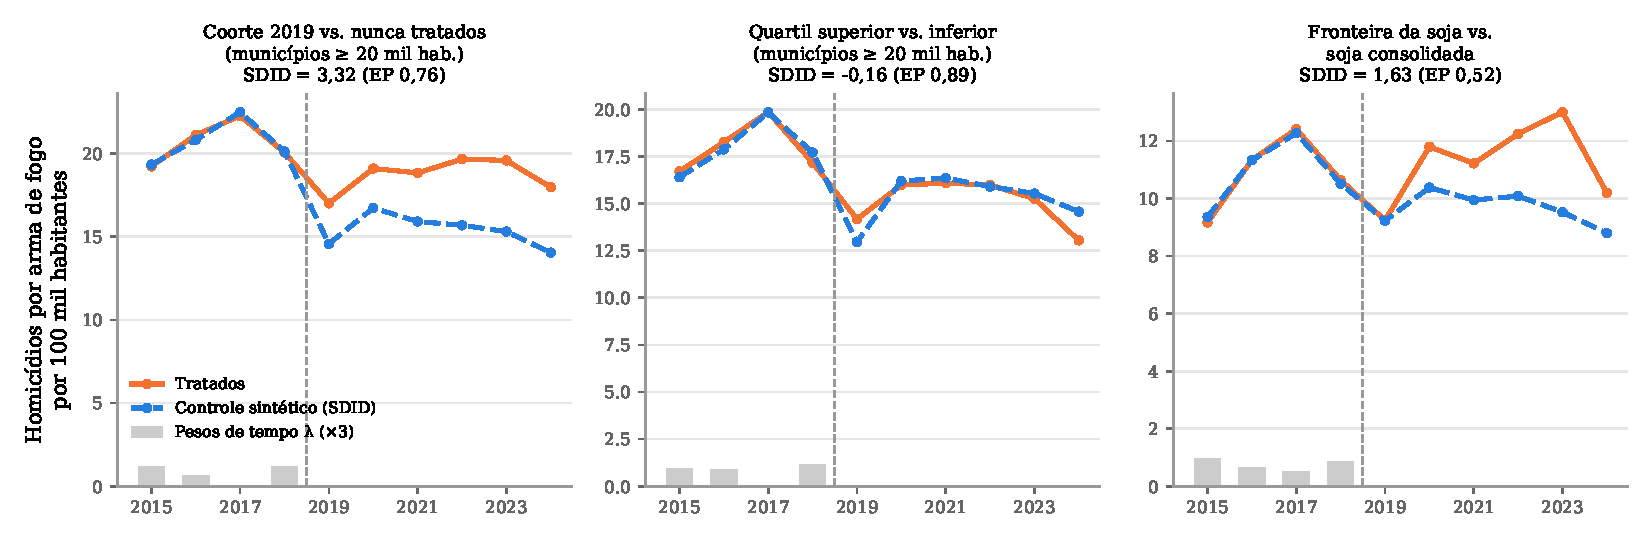
\includegraphics[width=\linewidth]{figs/sdid_pt.pdf}
\caption{SDID: trajetórias dos municípios tratados e dos controles sintéticos}\label{fig:sdid}
\nota{Linhas tracejadas representam o controle sintético do SDID, e as barras cinzas, os pesos de tempo.}
\end{figure}

\section{A fronteira da soja}\label{sec:soja}

A fronteira da soja reúne os municípios com ao menos 1.000 hectares de soja em 2018, área plantada pelo menos 50\% maior que a de 2010 e desmatamento entre 2015 e 2018 acima da mediana nacional. Esses critérios identificam 472 municípios, concentrados no Rio Grande do Sul, em Mato Grosso, no Tocantins, em Goiás, em Minas Gerais, em Santa Catarina e no Maranhão. Os grupos de comparação são os 1.105 produtores de soja consolidados e os 3.993 municípios sem produção relevante. A Tabela~\ref{tab:soja} mostra que a fronteira da soja recebeu mais armas após 2019 nas duas comparações. Contra os municípios sem soja, a diferença em diferenças indica 4{,}69 homicídios adicionais por 100 mil, mas o \textit{event study} revela uma tendência de alta anterior a 2019 (p do teste conjunto pré-tratamento igual a 0{,}027), compatível com a interiorização da violência.

Os estimadores que lidam com essa tendência confirmam o efeito. O SDID contra os produtores consolidados, comparação que isola a expansão recente entre municípios com a mesma base produtiva, estima 1{,}63 óbitos por 100 mil (erro-padrão de 0{,}52). Na versão escalonada do estimador de \citet{callaway2021}, em que cada município da fronteira entra no tratamento no ano de seu primeiro salto de registros (84 municípios em 2019, 153 em 2020 e 78 em 2021), o efeito é de 2{,}37 óbitos por 100 mil (erro-padrão de 0{,}80; p = 0{,}003), sem coeficientes pré-tratamento significativos e com resultado semelhante sob ponderação pela população. A tripla interação com a intensidade contínua indica que cada registro adicional tem efeito maior na fronteira da soja (0{,}35; p = 0{,}002), e os placebos com homicídios por arma branca são nulos. Na fronteira da soja, o efeito é, portanto, cerca de 45\% maior que a média nacional estimada pelo mesmo método. Esse desenho, contudo, não separa inteiramente a flexibilização das armas de outros choques do agronegócio no período, como a alta dos preços das \textit{commodities} entre 2020 e 2022; a evidência de que o canal opera pelas armas vem da maior expansão dos registros na fronteira e do efeito mais intenso por registro adicional.

\begin{table}[H]
\centering\footnotesize\setlength{\tabcolsep}{4pt}
\caption{A fronteira da soja como grupo tratado}\label{tab:soja}
\begin{tabular}{lcccc}
\toprule
 & \multicolumn{2}{c}{vs. sem soja} & \multicolumn{2}{c}{vs. soja consolidada} \\
\cmidrule(lr){2-3}\cmidrule(lr){4-5}
 & Coef. & EP & Coef. & EP \\
\midrule
Registros de armas por mil hab. (1º estágio) & 0{,}123$^{**}$ & (0{,}049) & 0{,}182$^{***}$ & (0{,}058) \\
DiD TWFE (ponderado pela pop.) & 4{,}693$^{***}$ & (1{,}168) & 1{,}147 & (1{,}193) \\
DiD TWFE (sem ponderação) & 2{,}441$^{***}$ & (0{,}503) & 1{,}395$^{***}$ & (0{,}533) \\
Event study: p do teste conjunto pré & 0{,}027 &  & 0{,}016 &  \\
SDID & 2{,}33$^{***}$ & (0{,}47) & 1{,}63$^{***}$ & (0{,}52) \\
SDID, tratados ponderados pela pop. & $-$0{,}34 & (0{,}97) & $-$1{,}14 & (0{,}99) \\
C\&S, bloco 2019 & 2{,}59$^{***}$ & (0{,}65) & 1{,}23$^{*}$ & (0{,}71) \\
C\&S, bloco 2019, ponderado & 2{,}92$^{**}$ & (1{,}24) & $-$0{,}61 & (1{,}15) \\
C\&S, escalonado pelo salto de registros & -- &  & 2{,}37$^{***}$ & (0{,}80) \\
C\&S, escalonado, ponderado & -- &  & 2{,}29$^{***}$ & (0{,}85) \\
\midrule
Placebo arma branca: DiD TWFE & $-$0{,}373 & (0{,}370) & $-$0{,}461 & (0{,}383) \\
Placebo arma branca: C\&S bloco & 0{,}32 & (0{,}42) & 0{,}67 & (0{,}48) \\
\midrule
Municípios tratados / controle & 472 / 3.993 &  & 472 / 1.105 &  \\
\bottomrule
\end{tabular}
\nota{Fronteira da soja: ao menos 1.000 ha de soja em 2018, área de soja 50\% maior que em 2010 e desmatamento entre 2015 e 2018 acima da mediana. DiD com efeitos fixos de município e de ano, controles e erros-padrão agrupados por município; SDID com erros-padrão por \textit{bootstrap} de municípios. Na versão escalonada do estimador de \citet{callaway2021}, as coortes são definidas pelo primeiro salto de registros, os controles são os produtores consolidados e os municípios ainda não tratados, e os municípios da fronteira sem salto são excluídos. $^{*}$ p$<$0,10; $^{**}$ p$<$0,05; $^{***}$ p$<$0,01. Fontes: IBGE/PAM, MapBiomas, SINARM/PF e SIM/DATASUS.}
\end{table}

\section{Discussão}\label{sec:discussao}

Os resultados alinham-se às evidências de \citet{duggan2001}, \citet{cook2006} e \citet{cerqueira2012}: a ampliação do estoque de armas legais em circulação elevou os homicídios por arma de fogo pelo canal de disponibilidade, sem contrapartida visível de dissuasão nas demais formas de homicídio. A magnitude é moderada. No estimador de \citet{callaway2021}, o efeito corresponde a cerca de 9\% da taxa média, e ocorreu em um período de queda nacional dos homicídios, de modo que a flexibilização não reverteu essa tendência, mas a atenuou nos municípios mais expostos. A ausência de reversão até 2024 é compatível com a permanência em circulação do estoque de armas acumulado entre 2019 e 2022.

A análise tem limitações. A medida de tratamento cobre as armas de posse de civis registradas na Polícia Federal e não inclui os CACs, cujos registros não são divulgados por município; o efeito estimado refere-se, portanto, à expansão da posse civil. O teste conjunto pré-tratamento do \textit{event study} convencional e o placebo com óbitos no trânsito sugerem que parte da associação pode refletir choques locais concomitantes, preocupação atenuada, mas não eliminada, pelos estimadores de \citet{callaway2021} e pelas especificações com controles de tendência. A causalidade reversa, em que municípios com violência crescente demandam mais armas, não pode ser descartada; um instrumento para a demanda local de armas anterior a 2019 seria um avanço. O SDID mostrou-se sensível ao grupo de comparação. Por fim, o desenho não distingue se os homicídios adicionais foram cometidos com armas registradas ou com armas desviadas para o mercado ilegal, e a hipótese de dissuasão sobre crimes patrimoniais não pôde ser testada por falta de dados municipais.

\section{Conclusão}\label{sec:conclusao}

Este artigo mostrou que a flexibilização do acesso a armas de fogo no Brasil entre 2019 e 2022 elevou os homicídios por arma de fogo nos municípios mais expostos ao choque. Cada novo registro de arma por mil habitantes aumentou a taxa de homicídios por arma de fogo em cerca de 0{,}225 óbitos por 100 mil ao ano, e os municípios que experimentaram um salto de registros registraram, em média, 1{,}62 óbitos adicionais por 100 mil. O efeito é específico às mortes por arma de fogo, mais intenso na fronteira da soja e persistente após a restrição de 2023. Do ponto de vista da política pública, os resultados indicam que a expansão da posse civil de armas tem um custo em vidas mensurável e duradouro, mesmo após a reversão normativa, porque o estoque acumulado permanece em circulação. A divulgação dos registros de CACs por município e a integração entre o SINARM e o SIGMA permitiriam avaliações mais completas.

\section*{Disponibilidade de dados e códigos}
Todos os dados utilizados são públicos. Os códigos de montagem do painel e de estimação estão disponíveis mediante solicitação ao autor correspondente.

\bibliographystyle{plainnat}
\bibliography{referencias}

\end{document}
